%!TEX root=../thesis.tex
\section{\acrshort{IEEE} 802.1AE \acrshort{MACsec}}
\label{sec:macsec}
The Standard for \acrfull{MACsec} has been published by the \gls{IEEE} in 2006~\cite{macsec}.
\gls{MACsec} is a protocol on layer 2 that provides confidentiality, integrity and data origin authenticity to mitigate network attacks.
Furthermore, it prevents replay attacks.

\subsection{Process}
The entity which is operating \gls{MACsec} is named \gls{SecY}.
For the operation of \gls{MACsec} cryptographic keys are needed because symmetric encryption and message authentication codes are used.
The entity that provides these is the \gls{KaY}.
How the \gls{KaY} works is not specified in the \gls{MACsec} standard but in IEEE 802.1X~\cite{ieee-802-1-x}.
It discovers other \glspl{KaY} that are attached to the same \gls{LAN}, mutually authenticates and authorizes them.
Thereby secure relationships are created, which the \gls{KaY} maintains.
The participants of these secure relationships form one \gls{CA}.
A \gls{SecY} can only be a member of one \gls{CA}.

The \gls{CA} is a group of \glspl{SecY}.
All members of a \gls{CA} use the same cipher suite, which defaults to GCM-AES-128.
With the amendment of 2011 GCM-AES-256 was added~\cite{macsecamendment1}.
The communication of the \gls{CA} members takes place through \glspl{SC}.

A \gls{SC} is a channel from one to many members within a \gls{CA}.
\glspl{SC} support the secure frame transmission using symmetric cryptography.
To distinguish different \glspl{SC} every \gls{SC} has an \gls{SCI}.
A \gls{SC} is supported by successive \glspl{SA}.

Each \gls{SA} uses an individual \gls{SAK}, which is provided by the \gls{KaY}.
To replace the cryptographic keys on a regular basis, the \gls{SecY} can replace a \gls{SA} with its successor.
To identify the used \gls{SA} the \gls{SCI} and an \gls{AN} are used.

\begin{figure}
  \centering
  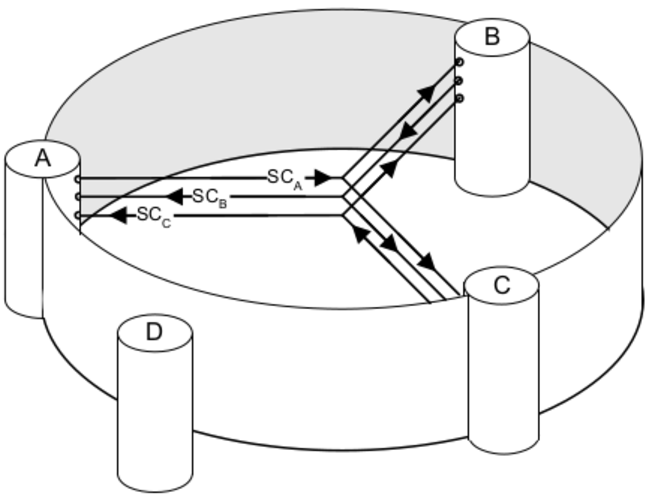
\includegraphics[width=0.8\columnwidth]{./ca-figure.pdf}
  \caption[\acrshort{MACsec} participants form a \acrshort{CA}]{The three stations A, B and C form one \acrlong{CA}.
  This \gls{CA} is supported by three \acrlongpl{SC}, \gls{SC}\textsubscript{A}, \gls{SC}\textsubscript{B} and \gls{SC}\textsubscript{C}.
  Station D has no secure connection to the other stations.\\
  Figure from the \gls{MACsec} standard~\cite[p.25]{macsec}}
  \label{fig:macsec-explanation}
\end{figure}

Figure~\ref{fig:macsec-explanation} displays four stations which are attached to the same \gls{LAN}.
Three of them build a \gls{CA}, which was established by \glspl{KaY}.
For secure communication three \glspl{SC} are build.
The cryptographic key which is used on each \gls{SC} depends on the current \gls{SA}.

\subsection{\acrlong*{MPDU}}
\label{sec:mpdu}
\gls{MACsec} works on a frame-by-frame basis.
To provide connectionless confidentiality, integrity, origin authenticity and to mitigate replay attacks, the Ethernet frame is modified.
The entities using \gls{MACsec} have to be attached on the same \gls{LAN} as it works on layer 2.

Furthermore, an \gls{ICV} is appended, to detect modifications and, therefore, protect the integrity of the \gls{SecTAG} and payload.

The structure of a \gls{MACsec} frame is shown in figure~\ref{fig:MPDU}.
As it is a modified Ethernet frame just the new fields are discussed, which are:
\begin{itemize}
  \item \acrlong{SecTAG} (8 or 16 bytes)
  \item Secure Payload
  \item \acrlong{ICV} (8 or 16 bytes)
\end{itemize}

\begin{figure}
  \centering
  %\definecolor{lightgray}{gray}{0.9}
  \begin{bytefield}[bitwidth=0.03\columnwidth]{12}
    \bitbox{4}{Preamble} & \bitbox{4}{Dest.} & \bitbox{4}{Source} \\
    \colorwordbox{pastelgreen}{1}{\acrlong{SecTAG}} \\
    \colorwordbox{pastelgreen}{3}{Secure Payload} \\
    %\skippedwords \\
    %\wordbox[lrb]{1}{} \\
    \colorwordbox{pastelgreen}{1}{\acrlong{ICV}} \\
    \wordbox{1}{Checksum}
  \end{bytefield}
  \caption[Basic \acrshort{MPDU} structure]{\acrlong{MPDU} (green) encapsulated in Ethernet frame.}
  \label{fig:MPDU}
\end{figure}

\subsubsection{\acrlong{SecTAG}}
The \gls{SecTAG} is displayed in~\ref{fig:sectag} and comprises of
\begin{itemize}
  \item MACsec Ethertype (2 bytes constant value 0x88E5)
  \item \acrfull{TCI} (6 bit)
  \item \acrfull{AN} (2 bit)
  \item \acrfull{SL} (1 byte)
  \item \acrfull{PN} (4 byte)
  \item \acrfull{SCI} (8 byte, optional)
\end{itemize}

\begin{figure}
  \centering
  \begin{bytefield}[bitwidth=0.0625\columnwidth]{8}
    \bitheader{1-8} \\
    \wordbox{2}{Ethertype 0x88E5} \\
    \bitbox{1}{V=0} & \bitbox{1}{ES} & \bitbox{1}{SC} & \bitbox{1}{SCB} & \bitbox{1}{E} & \bitbox{1}{C} & \bitbox{2}{\acrshort{AN}} \\
    \bitbox{6}{\acrshort{SL}} & \colorbitbox{lightgray}{2}{} \\
    \wordbox{4}{\acrshort{PN}} \\
    \begin{rightwordgroup}{optional}
      \wordbox[lrt]{1}{SCI}\\
      \skippedwords \\
      \wordbox[lrb]{1}{}
    \end{rightwordgroup}\\
  \end{bytefield}
  \caption[\acrshort{SecTAG} of an \acrshort{MPDU}]{\gls{SecTAG} of an \acrlong{MPDU}.}
  \label{fig:sectag}
\end{figure}

\pagebreak
The \gls{TCI} field comprises of the following bits:
\begin{itemize}
  \item Bit 1: Version (0 for~\cite{macsec})
  \item Bit 2: MAC Source Address parameter bit (set if the first 6 bytes of the source address are equal to \gls{SCI})
  \item Bit 3: Explicit \gls{SCI} bit (set if \gls{SCI} is encoded)
  \item Bit 4: Usage of EPON Single Copy Broadcast without explicit \gls{SCI} bit
  \item Bit 5: Encryption bit (set if secure payload is encrypted)
  \item Bit 6: Changed-Text bit (set if secure payload is not equal to payload of \gls{SDU})
  % Manche Integritätsverfahren hängen bspw. Daten an oder modifizieren sie, sodass die Nutzdaten dekodiert werden müssen, obwohl keine Verschlüsselung genutzt wurde
\end{itemize}

The two bit \gls{AN} is needed to identify different \gls{SA}, which needs to be known use the correct cryptographic key.

If the length of the secure payload is shorter than 48 bytes, the \gls{SL} field describes the length.
Otherwise it is null.
This is needed because frames that undercut the minimum ethernet frame size are padded.
If this happens, the receiver needs the length of the secure payload to locate the \gls{ICV}.
The seventh and eighth bit are currently not used and always zero.

To provide protection from replay attacks the \gls{PN} is an incrementing value for each frame secured with \gls{MACsec}.
Moreover, it is part of the \gls{IV} for the Cipher Suite, which is needed for confidentiality and integrity, concatenated with the \gls{SCI}. %Damit ist er predictable, oder? SaC I!

The \gls{SCI} is used to identify the \gls{SA} in combination with the \gls{AN}.
Moreover, it is needed to identify the \gls{SecY} which sent the frame in the network.
If the \gls{SecY} uses a point-to-point connection the use of the \gls{SCI} is not necessary.

\subsubsection{Secure Payload}
The secure payload field contains the unencrypted or encrypted data of the \gls{SDU}, depending on the configuration of \gls{MACsec}.
It's integrity is always protected, independent of whether encryption is configured or not.

\subsubsection{\acrlong{ICV}}
The \gls{ICV} is a message authentication code, therefore, it is used to verify the integrity of the whole frame.
It can be 8 bytes and 16 bytes long, this depends on the used cipher suite.
The calculation of the \gls{ICV} includes the source- and destination address, the \gls{SecTAG} and the secure payload.
